\documentclass[conference]{IEEEtran}
\IEEEoverridecommandlockouts
% The preceding line is only needed to identify funding in the first footnote. If that is unneeded, please comment it out.
\usepackage{cite}
\usepackage{amsmath,amssymb,amsfonts}
\usepackage{algorithmic}
\usepackage{graphicx}
\usepackage{textcomp}
\usepackage{xcolor}
\def\BibTeX{{\rm B\kern-.05em{\sc i\kern-.025em b}\kern-.08em
    T\kern-.1667em\lower.7ex\hbox{E}\kern-.125emX}}
\begin{document}

\title{Implementation and verification of a data vault\\\Large Storing and Managing Data (Module 06-32245), Autumn 2022}

\author{\IEEEauthorblockN{Jawali, Vijay, 2437649}
VXJ250@student.bham.ac.uk\\%Do not modify this line
\today}
%\and
%\IEEEauthorblockN{2\textsuperscript{nd} Given Name Surname}
%\IEEEauthorblockA{\textit{dept. name of organization (of Aff.)} \\
%Signal Processing, Autumn 2020, Course Research Project\\%Do not modify this line
%author email address}


\maketitle

\begin{abstract}
As the adoption of technology increases and companies continue to expand their business in this sphere, the amount of data generated by users will only increase. However, the data collected is heterogeneous and has to be converted into organised information that forms the basis of reporting and aids in decision-making. Data vault illustrates the implementations and steps to gather data from multiple sources and make it available in the form of a unified information store to serve clients' needs. Data vaults allow the agile development approach to build an enterprise warehouse that is capable of historical data tracking and enables auditing. This is implemented in tiers of Staging, Enterprise data warehouses and Reporting. Instead of focusing on a single topic for analysis, an enterprise data warehouse aims to represent all of the business data and business rules of an organisation. Following that, the information in the warehouse is presented so that business users can access all pertinent subject areas from individual data marts that contains a subset of the information kept by the business in a larger storage system.
\end{abstract}

\section{Introduction}\label{sec:Intro}
Any organisation now considers information to be a valuable resource to be able to make informed decisions and contribute value to the organization. Data vault enables them to achieve this goal for multiple use cases by using data valut having multiple tiers. Every function or department of an organisation has various demands for the data to be studied, so the enterprise data warehouse must offer a variety of subject areas to satisfy those needs. The information that is relevant to the user is contained in each subject area called data mart.

The Enterprise Data Warehouse design have evolved thanks to the Data Vault data model proposed by Linstedt ``Fig.~\ref{fig1}'' as an alternative to Inmon's and Kimball's traditional data warehouse architecture's. According to Linstedt, the 3NF of Inmon and the dimensional modeling of Kimball have weaknesses if the data volume increases \cite{b1}.Dan Linstedt defines the Data Vault as “a detail-oriented, historical tracking and uniquely linked set of normalized tables that support one or more functional areas of business”.

\begin{figure}[htbp]
\centerline{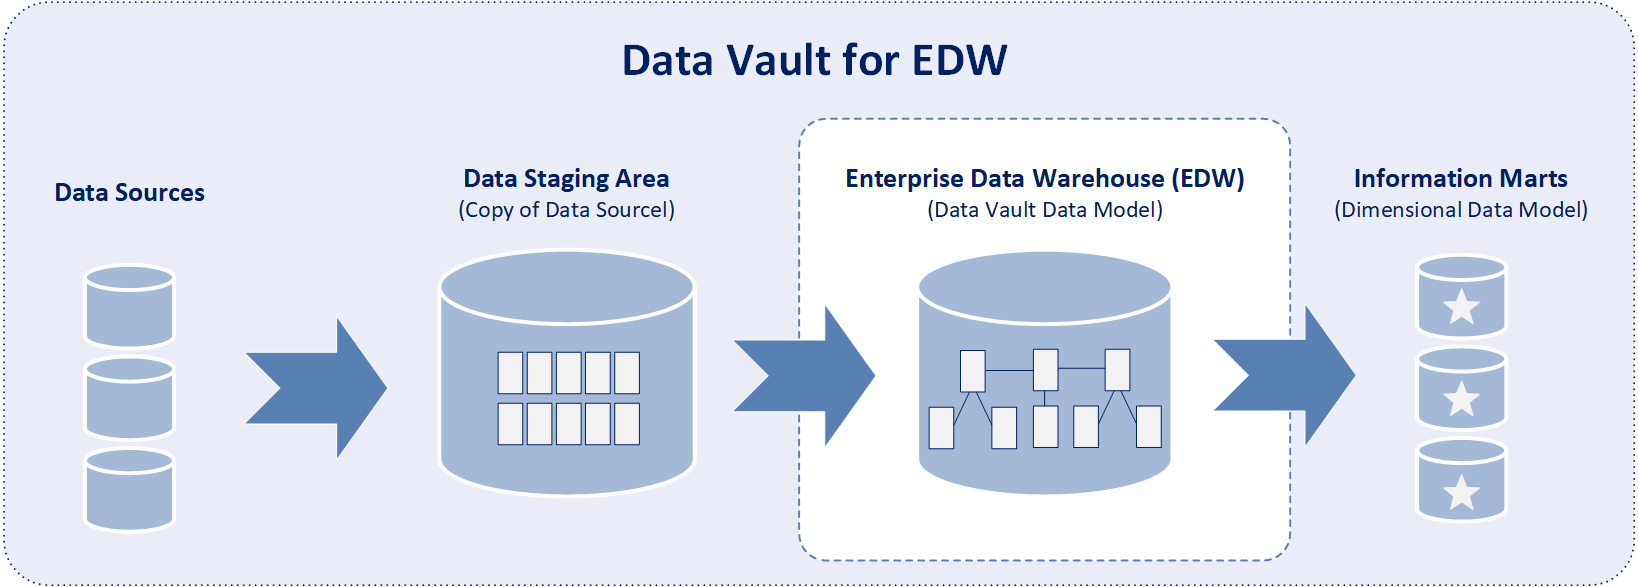
\includegraphics[width=9cm, height=4cm]{Figure1.png}}
\caption{Data Vault Architecture}
\label{fig1}
\end{figure}

\subsection{Staging Layer}

Before the data is imported to the data warehouse for analysis, a staging layer is a place for the loading and processing of source data. The staging area is used to aggregate data from various data sources, undergo transformations once data has been placed into it. At the staging area, ETL processing is executed.

\smallskip
\noindent ETL Process contains three steps:

\begin{enumerate}
\item Extract
\item Transform
\item Load
\end{enumerate}

\textbf{Extract} comprises gathering the information from various data sources that will be used to populate the Data Warehouse.

\textbf{Transform} receives data from extract stage and makes data ready to load in Enterprise Data Warehouse. In Data vault,data are segregated into Hubs, Links and Satellites. The data received is logically divided into pieces suitable to load according to enterprise entities. Therefore, each section of data will be divided during the transform step and then reorganised into a format that is consistent with the database design.

\textbf{Load} receives transformed data to insert it into data vault. Business key, the identity of the person inserting the data, is added to the data during the ETL process together with the current timestamp.

\subsection{Enterprise Data Warehouse Layer}

The model ``Fig.~\ref{fig2}'' represents business processes and is tied to business through business keys. This is an important property of the Data Vault model because business keys indicate how businesses integrate, connect, and access information in their systems. With the orientation of the Data Vault model on business keys, we inherit the ability to integrate, connect, and access information in the same manner as the business does in its daily operations \cite{b2}.

\begin{figure}[htbp]
\centerline{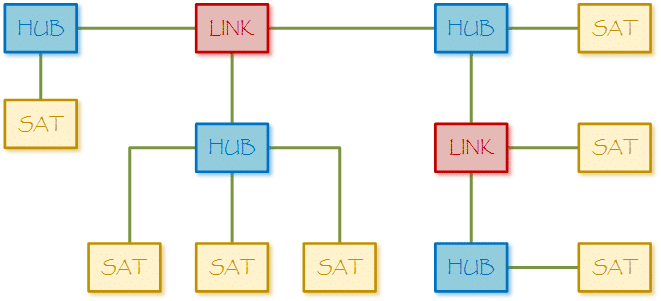
\includegraphics[width=9cm, height=4cm]{Figure2.png}}
\caption{Enterprise Data Warehouse Components}
\label{fig2}
\end{figure}

\smallskip
\noindent A Data Vault architecture is comprised of three main structures:

\begin{enumerate}
\item Hub
\item Link
\item Satellite
\end{enumerate}

A distinct set of business keys that describe fundamental business concepts acts as a \textbf{hub}. These distinct business keys are required to identify the information and business users use these to refer to the business objects when requesting information from an operational system.There are hubs for each area of business information in a Data Vault model.

Each business object interacts with the others in some way.They are linked together by the operational business processes, which employ business objects to carry out their functions. These connections are modelled by the Data Vault using a \textbf{link} that join two or more hubs.

A \textbf{satellite} is a table with extensive descriptive data that places the business keys from the Hub or Link in proper perspective. There can only be one parent table per satellite. Whenever changes to the data warehouse's descriptive data occur, it collects them with new timestamp that represents a newer version.

\subsection{Information delivery layer}

Data Vault 2.0 modelling is unfamiliar to the majority of business customers.In order to obtain useful and useable raw data that can be utilised for processing into usable information, they also need to be able to grasp how to combine the numerous entities. An information mart ``Fig.~\ref{fig3}'' is often used by end users to obtain prepared information that they can immediately utilise for the task at hand. As a means of user services, this layer queries about the enterprise layer. Data Marts are designed in start schema each of which exposes a portion of the vault for a certain user group. Hubs and their satellites often create dimensions, whereas linkages and their satellites create facts.

\begin{figure}[htbp]
\centerline{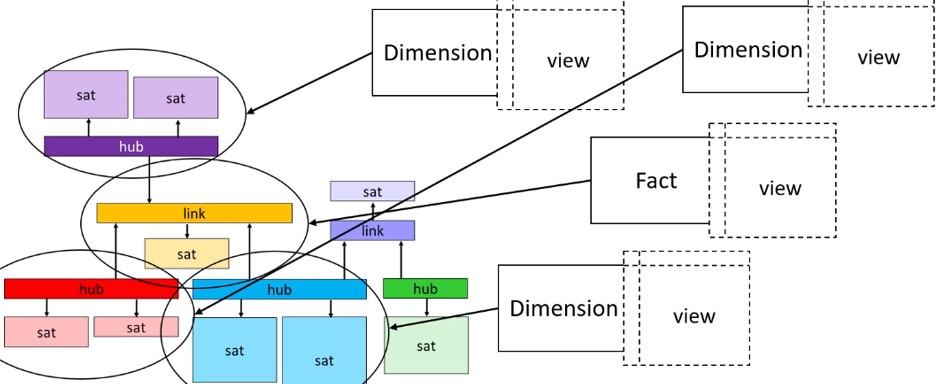
\includegraphics[width=9cm, height=4cm]{Figure3.png}}
\caption{Virtualized Information Mart}
\label{fig3}
\end{figure}


\section{State of the art of data vaults}


\section{Methods}

Raw data is received from multiple domains having different source systems, Initially, the data is read from the source systems and put in a staging area. A python program reads the data repository and collects information in raw format. It reads the metadata and stores it in a dictionary. Each of the dictionary values represents a key, value pair. Then the data is read in a two-dimensional array format. The next step in staging is to transform the raw format. A staging region that does not apply any modifications to the data or store historical information. In the transformation, the data are segregated into Links, Hubs, and satellites. Sequence keys are generated at this stage that uniquely describes the records in hubs and satellites. In addition to the sequence, the username of the person inserting data and timestamps are added to audit the data. Each of individual tables are created fed into postgres from python using postgres connectors that loads the data.

Enterprise Data Vault is implemented in postgres. A database is created and populated with Hubs that connect the satellite tables in the domain. Each of the satellite table must be linked to a Hub. Multiple Hubs are connected with Link tables that join the concurrent domains that are related to each other. Hubs only include a discrete list of business keys and information describing where and when each key was loaded. Satellites have information about their parent Hub or Link, as well as metadata indicating when and where the data was loaded,in addition to the domain information. There is no descriptive data element in links. The description section is in the satellites of Hubs. The only entity type that contains connections between Hubs are Links.

\smallskip
\noindent
\textbf{Business Keys:} Business keys provide an identity to data residing in Hubs. Naturally business keys should be chosen such that they are unique withing an Object defined by Hub. The scope of business key is limited to a hub, beyond that, other hubs within the same Opeational sysyem could have the same business keys. The larger the scope, the better it can represent the business object \cite{b3}.

\begin{figure}[htbp]
\centerline{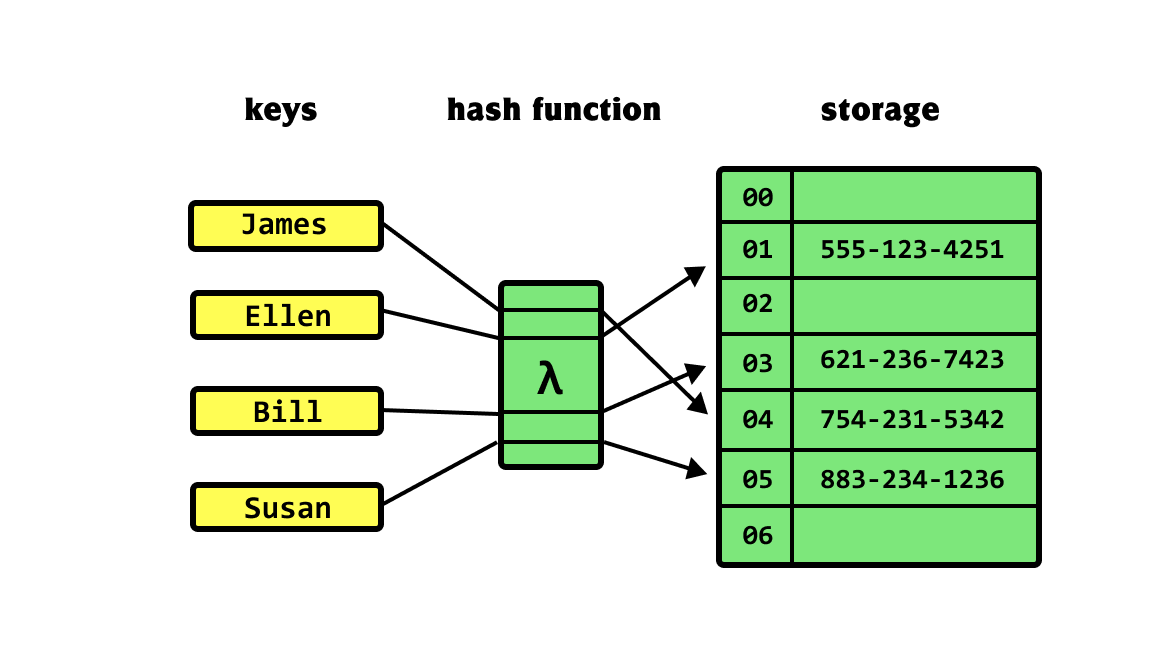
\includegraphics[width=9cm, height=4cm]{Figure4.png}}
\caption{Hashing Example}
\label{fig4}
\end{figure}

\smallskip
\noindent
\textbf{Hashing:} The hash key in a Data Vault hub is used to improve the lookup performance within a data warehouse built with the Data Vault \cite{b4}. This comes in handy when querying the final Data Vault model necessitates many more joins than querying a typical database. In addition to performance, hashing ``Fig.~\ref{fig4}'' provides a layer of security. hash keys are calculated with building MD5 algoritm.

\smallskip
\noindent
\textbf{Agile:} The Enterprise Layer of the Data Vault need not be designed completely in one go. A specific domain requirement that has priority could take up as a modular part. Hubs, Satellites and links are built. A Data Mart of this specific domain is created and insights are derived from Data Mart from limited Domains. As the requirement increases further, Data Vault will be scaled up to add new domains to serve a different use case. It provides us the ability for a Continuous development lifecycle with regular deliverables added and supported in an agile way.

\begin{figure}[htbp]
\centerline{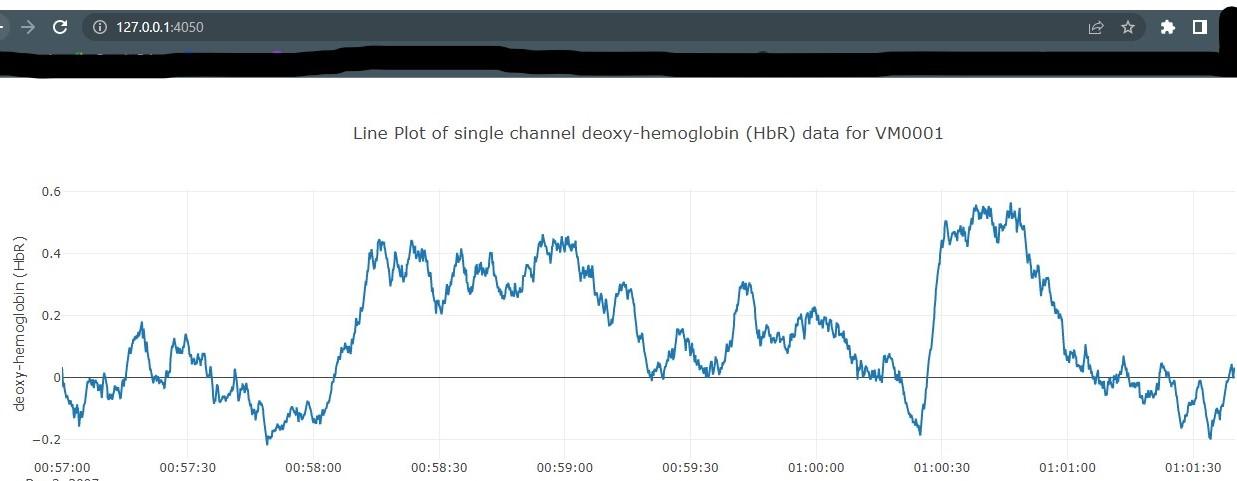
\includegraphics[width=9cm, height=4cm]{Figure5.png}}
\caption{Browser based GUI Interface Example}
\label{fig5}
\end{figure}

Information to end users is provided from data mart in the form of views. Dimensional modelling, often known as Kimball's star schema is used. Star Schema has two types of tables, Fact Table and Dimension Table. Fact tables include information about certain business processes or events that occur inside these processes. They provide reference to each Dimension. Fact tables may also contain measure which are numerical quantifiable values. Dimensions gives meaning when joined with fact Tables. They are critical to the data warehouse's understanding as all descriptive information is taken from the dimension tables. They can also be used to filter facts based on the dimensions themselves or one of their descriptive qualities. 

Additionally, aggregated measurements can be sorted by dimension or one of its properties. Providing facts and dimensions using virtualized approaches is more agile and responsive to user requests than ETL-based integration. These approaches require no data
moving or data materialization and are far easier to design and develop \cite{b5}. A browser based intuititive GUI ``Fig.~\ref{fig5}'' for querying is implemented using plotly that receives data from virtualized data marts and visualized them using graphs and charts accessible to users unfamiliar with querying.


\section{Results}

Metadata from the raw data is extracted from raw files and added to a dictionary variable, metadata ``Fig.~\ref{fig6}'' can comprise various datatypes that need to be extracted. To preserve the data types, data is loaded in postgres using a binary stream and encoded. Maintaining the object datatypes allows us to operate on them during the data retrieval stage. Data values are followed by metadata, they are retrieved in a structural format using libraries that read data in tabular such as pandas.

\begin{figure}[htbp]
\centerline{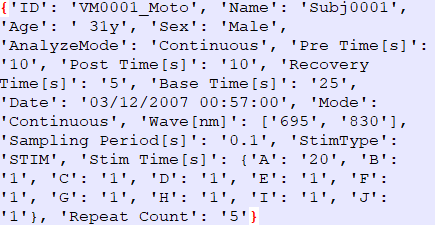
\includegraphics[width=9cm, height=4cm]{Figure6.png}}
\caption{Sample metadata Extraction in text format}
\label{fig6}
\end{figure}

Data along with metadata are loaded in postgres tables, the current timestamp, username is added and sequence key is hashed. postgres tables are validated whether data has been inserted.


Satellite Tables contain a part of descriptive information, while Hubs ``Fig.~\ref{fig7}'' connect the satellites ``Fig.~\ref{fig8}'' and in-turn multiple hubs are connected by Links ``Fig.~\ref{fig9}''.

\begin{figure}[htbp]
\centerline{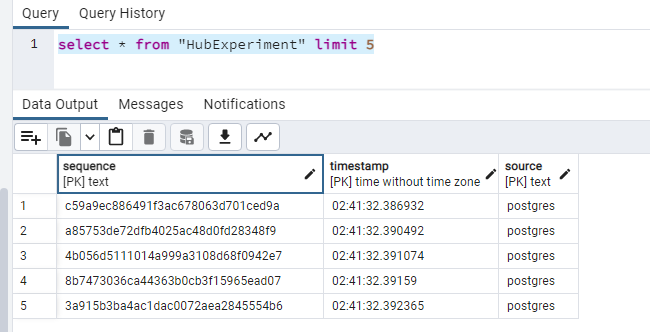
\includegraphics[width=9cm, height=4cm]{Figure7.png}}
\caption{Hub Data Example}
\label{fig7}
\end{figure}

\begin{figure}[htbp]
\centerline{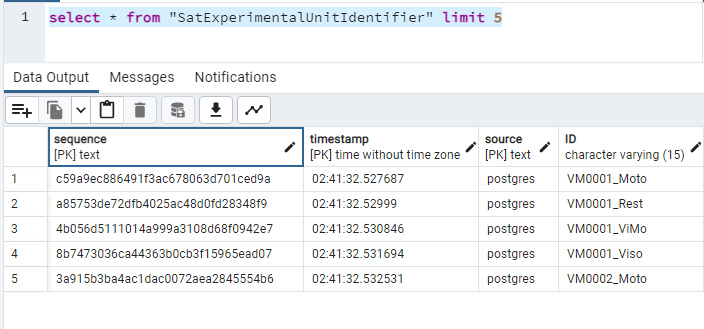
\includegraphics[width=9cm, height=4cm]{Figure8.png}}
\caption{Satellite Data Example}
\label{fig8}
\end{figure}

\begin{figure}[htbp]
\centerline{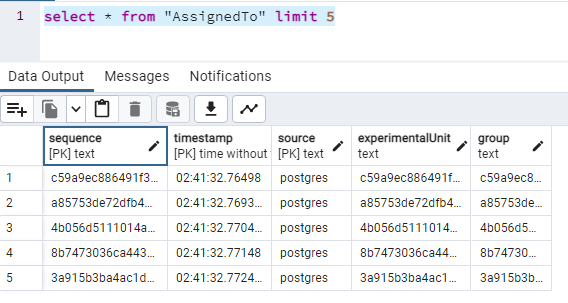
\includegraphics[width=9cm, height=4cm]{Figure9.png}}
\caption{Link Data Example}
\label{fig9}
\end{figure}

The data from Enterprise data vault are consumed by Information marts, Each information serves a business purpose and are characterized by fact and dimension tables. These are in the form of views ``Fig.~\ref{fig10}''.

\begin{figure}[htbp]
\centerline{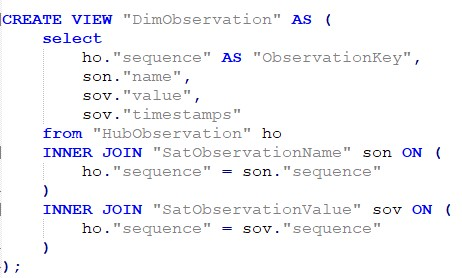
\includegraphics[width=9cm, height=4cm]{Figure10.png}}
\caption{Sample Dimenaion View}
\label{fig10}
\end{figure}

Final layer will be GUI layer layer that consumes data from Data mart and visualizes them in graphical ``Fig.~\ref{fig11}'' form. In this section the user has the ability to choose the data he needs to view. Drop-down options are provided to browse a particular experiment.


\begin{figure}[htbp]
\centerline{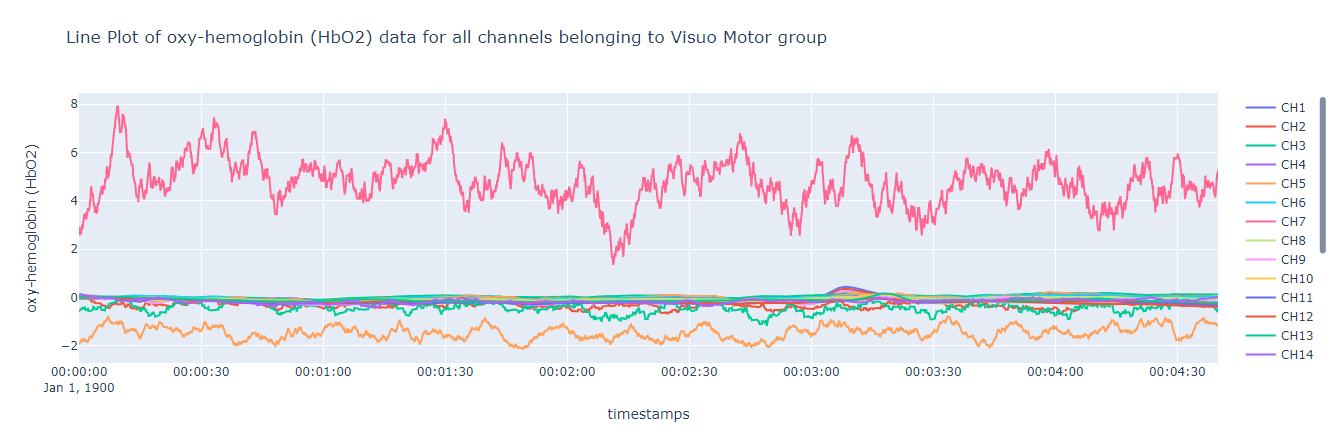
\includegraphics[width=9cm, height=4cm]{Figure11.png}}
\caption{Example Graphical GUI charts}
\label{fig11}
\end{figure}









\textcolor{red}{This template contain guidance text for composing and formatting your semester project report. Please ensure that all template text is removed from your report prior to submission to the lecturer. Failure to remove the template text from your report may result in your marks being unnecessarily low.}

\section{Ease of Use}

\subsection{Maintaining the Integrity of the Specifications}

The IEEEtran class file is used to format your report and style the text. All margins, 
column widths, line spaces, and text fonts are prescribed; please do not 
alter them. You may note peculiarities. For example, the head margin
measures proportionately more than is customary. %This measurement and others are deliberate, using specifications that anticipate your paper as one part of the entire proceedings, and not as an independent document. 
Please \textbf{do not revise any of the current designations}.

\section{Prepare Your Report Before Styling}
Before you begin to format your report, first write and save the content as a separate text file. Complete all content and organizational editing before formatting. Please note sections \ref{AA}--\ref{SCM} below for more information on 
proofreading, spelling and grammar.

Keep your text and graphic files separate until after the text has been 
formatted and styled. Do not number text heads---{\LaTeX} will do that for you.

\subsection{Abbreviations and Acronyms}\label{AA}
Define \emph{all} abbreviations and acronyms the first time they are used in the text, even after they have been defined in the abstract. %Abbreviations such as IEEE, SI, MKS, CGS, ac, dc, and rms do not have to be defined.
Do not use abbreviations in the title or heads unless they are unavoidable.

\subsection{Units}
\begin{itemize}
\item Use either SI as primary units. %English units may be used as secondary units (in parentheses). An exception would be the use of English units as identifiers in trade, such as ``3.5-inch disk drive''.
%\item Avoid combining SI and CGS units, such as current in amperes and magnetic field in oersteds. This often leads to confusion because equations do not balance dimensionally. If you must use mixed units, clearly state the units for each quantity that you use in an equation.
\item Do not mix complete spellings and abbreviations of units: ``Wb/m\textsuperscript{2}'' or ``webers per square meter'', not ``webers/m\textsuperscript{2}''. Spell out units when they appear in text: ``. . . a few henries'', not ``. . . a few H''.
\item Use a zero before decimal points: ``0.25'', not ``.25''. Use ``cm\textsuperscript{3}'', not ``cc''.)
\end{itemize}

\subsection{Equations}
Number equations consecutively. To make your equations more compact, you may use the solidus (~/~), the exp function, or appropriate exponents. Italicize Roman symbols for quantities and variables, but not Greek symbols. Use a long dash rather than a hyphen for a minus sign. Punctuate equations with commas or periods when they are part of a sentence, as in:
\begin{equation}
a+b=\gamma
\label{eq}
\end{equation}

Be sure that the symbols in your equation have been defined before or immediately following the equation. Use ``Eq.~\eqref{eq}'', not ``eqref{eq}'' or ``equation \eqref{eq}'', except at 
the beginning of a sentence: ``Equation~\eqref{eq} is . . .''

\subsection{\LaTeX-Specific Advice}

Please use ``soft'' (e.g., \verb|\eqref{Eq}|) cross references instead
of ``hard'' references (e.g., \verb|(1)|). That will make it possible
to combine sections, add equations, or change the order of figures or
citations without having to go through the file line by line.

Please don't use the \verb|{eqnarray}| equation environment. Use
\verb|{align}| or \verb|{IEEEeqnarray}| instead. The \verb|{eqnarray}|
environment leaves unsightly spaces around relation symbols.

Please note that the \verb|{subequations}| environment in {\LaTeX}
will increment the main equation counter even when there are no
equation numbers displayed. If you forget that, you might write an
article in which the equation numbers skip from (17) to (20), causing
the lecturer to wonder if you've discovered a new method of
counting.

{\BibTeX} does not work by magic. It doesn't get the bibliographic
data from thin air but from .bib files. If you use {\BibTeX} to produce a bibliography you must send the .bib files. 

{\LaTeX} can't read your mind. If you assign the same label to a
subsubsection and a table, you might find that Table I has been cross
referenced as Table IV-B3. 

{\LaTeX} does not have precognitive abilities. If you put a
\verb|\label| command before the command that updates the counter it's supposed to be using, the label will pick up the last counter to be
cross referenced instead. In particular, a \verb|\label| command
should not go before the caption of a figure or a table.

Do not use \verb|\nonumber| inside the \verb|{array}| environment. It will not stop equation numbers inside \verb|{array}| (there won't be any anyway) and it might stop a wanted equation number in the
surrounding equation.

\subsection{Some Common Mistakes}\label{SCM}
\begin{itemize}
\item The word ``data'' is plural, not singular. The singular is datum.
\item The subscript for the permeability of vacuum $\mu_{0}$, and other common scientific constants, is zero with subscript formatting, not a lowercase letter ``o''.
\item In American English, commas, semicolons, periods, question and exclamation marks are located within quotation marks only when a complete thought or name is cited, such as a title or full quotation. When quotation marks are used, instead of a bold or italic typeface, to highlight a word or phrase, punctuation should appear outside of the quotation marks. A parenthetical phrase or statement at the end of a sentence is punctuated outside of the closing parenthesis (like this). (A parenthetical sentence is punctuated within the parentheses.)
\item A graph within a graph is an ``inset'', not an ``insert''. The word alternatively is preferred to the word ``alternately'' (unless you really mean something that alternates).
\item Do not use the word ``essentially'' to mean ``approximately'' or ``effectively''.
\item In your paper title, if the words ``that uses'' can accurately replace the word ``using'', capitalize the ``u''; if not, keep using lower-cased.
\item Be aware of the different meanings of the homophones ``affect'' and ``effect'', ``complement'' and ``compliment'', ``discreet'' and ``discrete'', ``principal'' and ``principle''.
\item Do not confuse ``imply'' and ``infer''.
\item The prefix ``non'' is not a word; it should be joined to the word it modifies, usually without a hyphen.
\item There is no period after the ``et'' in the Latin abbreviation ``et al.''.
\item The abbreviation ``i.e.'' means ``that is'', and the abbreviation ``e.g.'' means ``for example''.
\end{itemize}
An excellent style manual for science writers is \cite{b7}.


\subsection{Identify the Headings}

The document must be structures according to the sections enumerated in Sect.~\ref{sec:Intro}. 
Within these major sections your are allowed to create subsections as needed.

\subsection{Figures and Tables}
\paragraph{Positioning Figures and Tables} Place figures and tables at the top and bottom of columns. Avoid placing them in the middle of columns. Large figures and tables may span across both columns. Figure captions should be below the figures; table heads should appear above the tables. Insert figures and tables after they are cited in the text. Use the abbreviation ``Fig.~\ref{fig}'', even at the beginning of a sentence. Do not abbreviate Table. Use ``Table.~\ref{tab1}'', even at the beginning of a sentence.

\begin{table}[htbp]
\caption{Table Type Styles}
\begin{center}
\begin{tabular}{|c|c|c|c|}
\hline
\textbf{Table}&\multicolumn{3}{|c|}{\textbf{Table Column Head}} \\
\cline{2-4} 
\textbf{Head} & \textbf{\textit{Table column subhead}}& \textbf{\textit{Subhead}}& \textbf{\textit{Subhead}} \\
\hline
copy& More table copy$^{\mathrm{a}}$& &  \\
\hline
\multicolumn{4}{l}{$^{\mathrm{a}}$Sample of a Table footnote.}
\end{tabular}
\label{tab1}
\end{center}
\end{table}

\begin{figure}[htbp]
\centerline{\includegraphics{fig1.png}}
\caption{Example of a figure caption.}
\label{fig}
\end{figure}

Figure Labels: Use 8 point Times New Roman for Figure labels. This is already set for you, so do not worry. Use words 
rather than symbols or abbreviations when writing Figure axis labels to avoid confusing the reader. As an example, write the quantity 
``Magnetization'', or ``Magnetization, M'', not just ``M''. If including 
units in the label, present them within parentheses. Do not label axes only with units. In the example, write ``Magnetization (A/m)'' or ``Magnetization \{A[m(1)]\}'', not just ``A/m''. Do not label axes with a ratio of quantities and units. For example, write ``Temperature (K)'', not ``Temperature/K''.

\section*{Acknowledgement}

Write the names of all those who help you to develop their project and describe their contibution in a single sentence. For instance, ``I would like to thank John Smith for providing helps with the mathematics of algorithm 1.''


\section*{References}

Please number citations consecutively within brackets \cite{b1}. The 
sentence punctuation follows the bracket \cite{b2}. Refer simply to the reference 
number, as in \cite{b3}---do not use ``Ref. \cite{b3}'' or ``reference \cite{b3}'' except at 
the beginning of a sentence: ``Reference \cite{b3} was the first $\ldots$''

Number footnotes separately in superscripts. Place the actual footnote at the bottom of the column in which it was cited. Do not put footnotes in the abstract or reference list. Use letters for table footnotes.

Unless there are six authors or more give all authors' names; do not use ``et al.''. Papers that have not been published, even if they have been submitted for publication, should be cited as ``unpublished'' \cite{b4}. Papers that have been accepted for publication should be cited as ``in press'' \cite{b5}. Capitalize only the first word in a paper title, except for proper nouns and element symbols.

For papers published in translation journals, please give the English 
citation first, followed by the original foreign-language citation \cite{b6}.

\begin{thebibliography}{00}
\bibitem{b1} G. Eason, B. Noble, and I. N. Sneddon, ``On certain integrals of Lipschitz-Hankel type involving products of Bessel functions,'' Phil. Trans. Roy. Soc. London, vol. A247, pp. 529--551, April 1955.
\bibitem{b2} J. Clerk Maxwell, A Treatise on Electricity and Magnetism, 3rd ed., vol. 2. Oxford: Clarendon, 1892, pp.68--73.
\bibitem{b3} I. S. Jacobs and C. P. Bean, ``Fine particles, thin films and exchange anisotropy,'' in Magnetism, vol. III, G. T. Rado and H. Suhl, Eds. New York: Academic, 1963, pp. 271--350.
\bibitem{b4} K. Elissa, ``Title of paper if known,'' unpublished.
\bibitem{b5} R. Nicole, ``Title of paper with only first word capitalized,'' J. Name Stand. Abbrev., in press.
\bibitem{b6} Y. Yorozu, M. Hirano, K. Oka, and Y. Tagawa, ``Electron spectroscopy studies on magneto-optical media and plastic substrate interface,'' IEEE Transl. J. Magn. Japan, vol. 2, pp. 740--741, August 1987 [Digests 9th Annual Conf. Magnetics Japan, p. 301, 1982].
\bibitem{b7} M. Young, The Technical Writer's Handbook. Mill Valley, CA: University Science, 1989.
\end{thebibliography}


\end{document}
